\documentclass{article}

\usepackage{tikz}
\usepackage{verbatim}
\usepackage{parskip}
\usepackage{amsthm}
\usepackage{xpatch}
\usepackage{amsmath}
\usepackage{graphicx}

\graphicspath{ {./img/} }

\setlength\parindent{0pt}

\newtheorem{definicija}{Definicija}[subsection]
\newtheorem{lema}{Lema}[subsection]
\newtheorem{izrek}{Izrek}[subsection]
\newtheorem{trditev}{Trditev}[subsection]
\newtheorem{posledica}{Posledica}[subsection]
\newtheorem{domneva}{Domneva}[subsection]
\newtheorem{primer}{Primer}[subsection]
\newtheorem{opomba}{Opomba}[subsection]

\makeatletter
\xpatchcmd{\@thm}{\thm@headpunct{.}}{\thm@headpunct{:}}{}{}
\makeatother

\begin{document}
\pagestyle{empty}

\begin{comment}
definitions
\end{comment}

%%%%%%%%%%%%%%%%%%%%%%%%%%%%%%%%%%%%%%%%%%%%%%%%%%%%%%%%%%%%%%%%%
\section{ Obseg in ploscina }
\subsection{ Večkotniki }

\begin{definicija}[Obseg]
    Obseg večkotnika je vsota dolžin njegovih stranic.
\end{definicija}

\begin{figure}[h]
    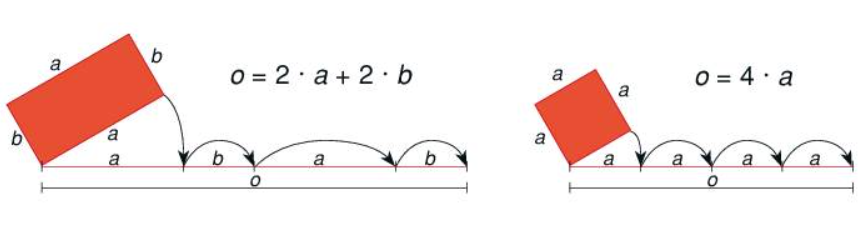
\includegraphics[width=\linewidth]{obsegPravokotnikInKvadrat.png}
    \centering
    \caption{Obseg pravokotnika in kvadrata.}
\end{figure}

\begin{definicija}[Ploščina]
    Ploščina večkotnika je število vseh ploščinskih enot, s katerimi je lik prekrit, ali pa vsota ploščin vseh pravokotnikov in kvadratov, na katere je večkotnik razdeljen.
\end{definicija}

\begin{figure}[h]
    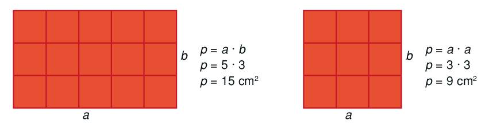
\includegraphics[width=\linewidth]{ploscinaPravokotnikInKvadrat.png}
    \centering
    \caption{Ploscina pravokotnika in kvadrata.}
\end{figure}
\begin{figure}[h]
    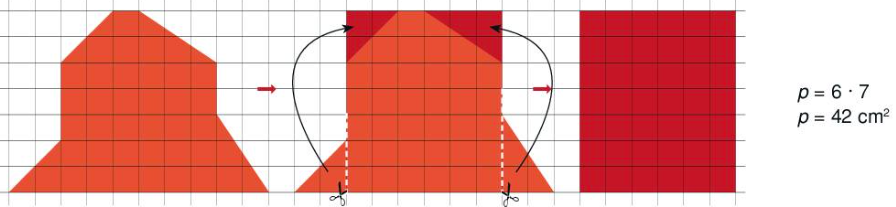
\includegraphics[width=\linewidth]{preoblikovanjeLikaVPravokotnik.png}
    \centering
    \caption{Izračun ploščine s preoblikovanjem lika v pravokotnik.}
\end{figure}

\pagebreak
\subsection{ Paralelogram }

\begin{trditev}[Obseg paralelograma]
    Obseg paralelograma je vsota dolžin vseh njegovih stranic.
    \[ o = 2 \cdot a + 2 \cdot b \]
\end{trditev}

\begin{trditev}[Ploščina paralelograma]
    Ploščina paralelograma je enaka produktu dolžine stranice in pripadajoče višine.
    \[ p = a \cdot v_a \quad \text{ali} \quad p = b \cdot v_b \]
\end{trditev}

\begin{figure}[h]
    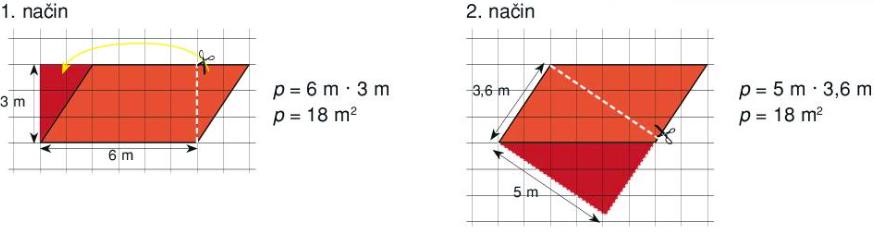
\includegraphics[width=\linewidth]{ploscinaPralelograma.png}
    \centering
    \caption{Izračun ploščine s preoblikovanjem paralelograma v pravokotnik.}
\end{figure}


\begin{trditev}[Obseg romba]
    Obseg romba je štirikratnik dolžine stranice.
    \[ o = 4 \cdot a \]
\end{trditev}

\begin{trditev}[Ploščina romba]
    Ploščina romba je enaka produktu dolžine stranice in višine.
    \[ p = a \cdot v_a \]
\end{trditev}

\begin{figure}[h]
    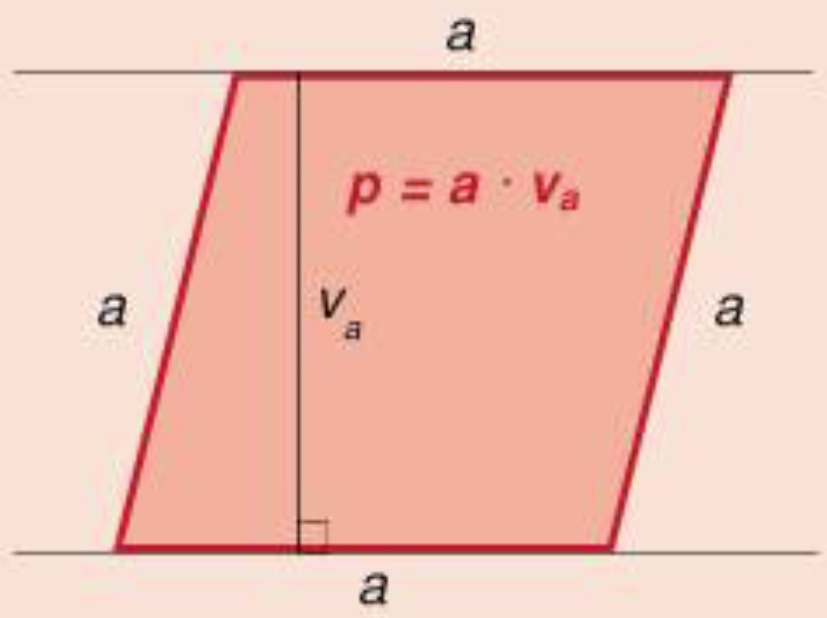
\includegraphics[width=0.3\linewidth]{ploscinaRomba.png}
    \centering
    \caption{Ploscina romba.}
\end{figure}

\pagebreak
\subsection{ Trikotniki }

\begin{trditev}[Obseg trikotnika]
    Obseg trikotnika je vsota dolžin vseh treh njegovih stranic.
    \[ o = a + b + c \]
\end{trditev}

\begin{trditev}[Ploščina trikotnika]
    Ploščina trikotnika je enaka polovici produkta dolžine poljubne stranice in pripadajoče višine.
    \[ p = \frac{a \cdot v_a}{2} = \frac{b \cdot v_b}{2} = \frac{c \cdot v_c}{2} \]
\end{trditev}

\begin{figure}[h]
    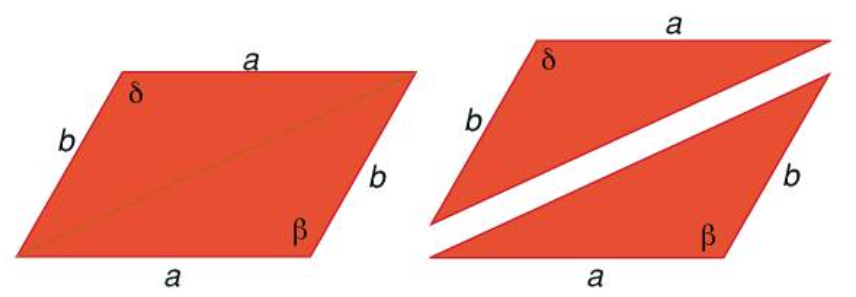
\includegraphics[width=\linewidth]{skladnaTrikotnikaParalelogram.png}
    \centering
    \caption{Dva skladna trikotnika ustvarita paralelogram.}
\end{figure}

\pagebreak
\subsection{ Deltoid, romb in kvadrat }

\begin{trditev}[Ploščina štirikotnika s pravokotnima diagonalama]
    Ploščina štirikotnika s pravokotnima diagonalama (kvadrat, pravokotnik, deltoid, romb) je enaka polovici produkta dolžin obeh diagonal.
    \[ p = \frac{e \cdot f}{2} \]
\end{trditev}


\begin{figure}[h]
    \includegraphics[width=\linewidth]{preoblikovanjeŠtirikotnikaSPravokotnimiDiagonalamiVPravokotnik.png}
    \centering
    \caption{Preoblikovanje deltoida v pravokotnik s stranicama e in f.}
\end{figure}

\pagebreak
\subsection{ Trapez }

\begin{trditev}[Ploščina trapeza]
    Ploščina trapeza je produkt dolžin srednice in višine. Ker je srednjica trapeza polovica vsote dolžin obeh osnovnic, je ploščina kar:
    \[ p = s \cdot v =  \frac{a + c}{2} \cdot v \]
\end{trditev}

\begin{figure}[h]
    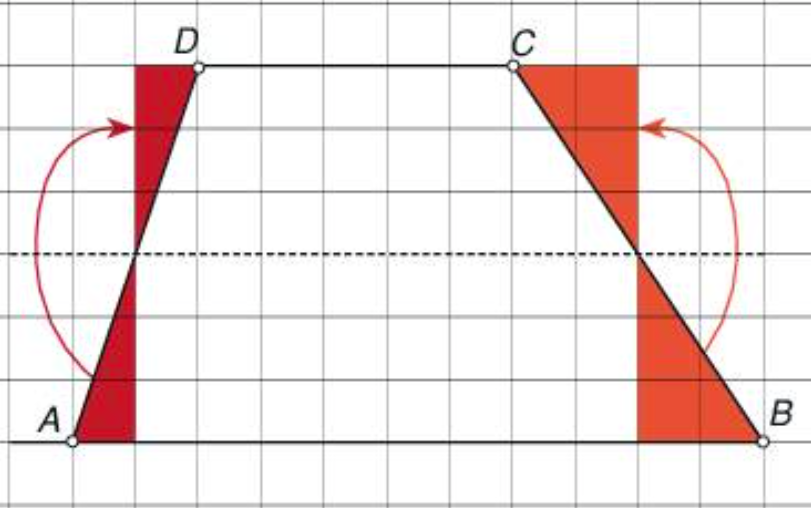
\includegraphics[width=\linewidth]{preoblikovanjeTrapezaVPravokotnik.png}
    \centering
    \caption{Preoblikovanje trapeza v pravokotnik s stranicama s in v.}
\end{figure}



\end{document}